% LaTeX-Vorlage zur Erstellung einer Abschlussarbeit in der Fakultät Elektrotechnik, Medien und Informatik an der OTH Amberg-Weiden
% Diese Vorlage entstand im Rahmen des Kurses "LaTeX fürs Studium"
% Aktuelle Version: v0.02
% Stand: 06.08.2015
%
% Changelog:
%
% v0.02: 06.08.2015, Anpassung der Vorlage:
% + Persönliche Informationen (Vorname, Name, Titel usw.) werden direkt in die PDF-Dokumenteinstellungen übernommen
% + Korrektur der Verlinkung von Abbildungs- und Tabellenverzeichnis aus dem Inhaltsverzeichnis (phantomsection) bzw. deren Seitenzahl
%   Besten Dank für diesen Hinweis an Jan-Olaf Becker
% + Anpassung des Namens der Fakultät nach deren Umbenennung
%
% v0.01: 14.03.2012, Erstellung der Vorlage

\documentclass[12pt,oneside]{report}
\usepackage[T1]{fontenc}		% Einstellungen fuer Umlaute usw.
\usepackage[utf8x]{inputenc}
\usepackage[ngerman]{babel}

\usepackage{parskip}			% Einstellungen fuer Absaetze: Abstand statt Einrueckung

\usepackage[a4paper,			% Papierformat A4
	    left=2.5cm,				% linker Rand
	    right=2.5cm,			% rechter Rand
	    top=1.5cm,				% oberer Rand
	    bottom=1.5cm,			% unter Rand
	    marginparsep=5mm,		% Abstand der Randnotizen
	    marginparwidth=10mm, 	% Breite der Randnotizen
	    headheight=7mm,			% Hoehe der Kopfzeile
	    headsep=1.2cm,			% Abstand der Kopfzeile
	    footskip=1.5cm,			% Abstand der Fusszeile
	    includeheadfoot]{geometry}

\usepackage{fancyhdr}						% Konfiguration von Kopf- und Fusszeilen
\pagestyle{fancy}							% Seitenstil 'fancy'
\fancyhf{}									% vorhandene Einstellungen loeschen
\setlength{\headwidth}{\textwidth}			% Kopf- und Fusszeile so breit wie der Haupttext
\fancyfoot[R]{\thepage} 					% Festlegung des Seitenstils: Seitenzahlen in der Fusszeile rechts
\fancyfoot[L]{\leftmark}					% Kapitelnr. und -Bezeichnung in der Fusszeile links
\fancyhead[R]{\IhreArbeit}					% "Bachelorarbeit" in der Kopfzeile rechts
\fancyhead[L]{\IhrVorname\ \IhrNachname}	% Vorname und Name in der Kopfzeile links
\renewcommand{\chaptermark}[1]{			% Definition der Ausgabe des Kapitels
  \markboth{Kapitel \thechapter. #1}{}}
\renewcommand{\headrulewidth}{0.5pt}		% Trennlinie zwischen Kopfzeile und Haupttext
\renewcommand{\footrulewidth}{0.5pt}		% Trennlinie zwischen Haupttext und Fusszeile
\fancypagestyle{plain}{					% Anpassung des Seitenstils 'plain' bei Beginn neuer Kapitel
  \fancyhf{}								% Vorbelegung loeschen
  \fancyfoot[C]{\thepage}					% Seitenzeilen in der Fusszeile mittig
  \fancyhead[R]{\IhreArbeit}				% "Bachelorarbeit" in der Kopfzeile rechts
  \fancyhead[L]{\IhrVorname\ \IhrNachname}	% Vorname und Name in der Kopfzeile links
}

\usepackage{amsmath}			% Pakete fuer den Mathematikmodus
\usepackage{amssymb}
\usepackage[intlimits]{empheq}

\usepackage[sc]{mathpazo}		% Schriftart Palatino fuer Haupttext und Mathematikmodus
\usepackage{pifont}				% zusaetzliche Symbole

\usepackage[format=hang,		% Einstellung fuer Bildunterschriften
            font={footnotesize},
            labelfont={bf},
            margin=1cm,
            aboveskip=5pt,
            position=bottom]{caption}

\usepackage{graphicx}							% Einbinden von Graphiken
\usepackage[svgnames,cmyk,table,hyperref]{xcolor} 	% Verwendung von Farben
\usepackage{tikz}								% Erstellen von Grafiken
\usetikzlibrary{positioning,arrows,plotmarks} % TikZ-Bibliotheken
%\usepackage{pgfplots}                           % Darstellung von Plots, Funktionen, Graphen usw.

%
% Weitere Pakete
%
%\usepackage{listings}			% Darstellung von Quellcode
%\lstset{language=Python, basicstyle=\ttfamily, numbers=none}
%
%\usepackage[european, siunitx]{circuitikz}	% Darstellung von Schaltungen
%
%\usepackage{enumerate}			% Formatierung nummerierter Listen

\usepackage{microtype,relsize}					% Wird verwendet, um Nachnamen auf Titelseite gesperrt darzustellen
\newcommand*{\Sperren}[1]{\textls*[100]{#1}}

% 
% Persoenliche Angaben
% 
\newcommand*{\Name}{Dominik}
\newcommand*{\Nachname}{Panzer}
\newcommand*{\Namezwei}{Manuel}
\newcommand*{\Nachnamezwei}{Pickl}
\newcommand*{\Namedrei}{Berkay}
\newcommand*{\Nachnamedrei}{Yurdagül}
\newcommand*{\IhrStudiengang}{Medieninformatik}
\newcommand*{\IhrFach}{Physical Computing}
\newcommand*{\IhreArbeit}{Wire \& Warriors}
\newcommand*{\IhrBearbeitungszeitraumVON}{26. April 2023}
\newcommand*{\IhrBearbeitungszeitraumBIS}{31. Juli 2023}
\newcommand*{\IhrErstpruefer}{Prof. Dipl.-Des. Martin Frey}
\newcommand*{\IhrZweitpruefer}{Prof. Dr.-Ing. Ulrich Schäfer}
\newcommand*{\IhrDrittpruefer}{Prof. Dr.-Ing. Gerald Pirkl}
\newcommand*{\IhreZusammenfassung}{%
Lorem ipsum dolor sit amet, consetetur sadipscing elitr, sed diam nonumy eirmod tempor invidunt ut labore et dolore magna aliquyam erat, sed diam voluptua. At vero eos et accusam et justo duo dolores et ea rebum. Stet clita kasd gubergren, no sea takimata sanctus est Lorem ipsum dolor sit amet. Lorem ipsum dolor sit amet, consetetur sadipscing elitr, sed diam nonumy eirmod tempor invidunt ut labore et dolore magna aliquyam erat, sed diam voluptua. At vero eos et accusam et justo duo dolores et ea rebum. Stet clita kasd gubergren, no sea takimata sanctus est Lorem ipsum dolor sit amet.
}
\newcommand*{\IhreSchluesselwoerter}{\LaTeX, Textsatz, Formeln, Graphiken}


\usepackage[bookmarks, raiselinks, pageanchor, % PDF-Einstellungen
            hyperindex, colorlinks,
            citecolor=black, linkcolor=black,
            urlcolor=black, filecolor=black,
            menucolor=black]{hyperref}
\hypersetup{pdftitle={\IhrTitelDE},%
            pdfauthor={\IhrVorname\ \IhrNachname},%
            pdfsubject={\IhreArbeit},%
            pdfkeywords={\IhreSchluesselwoerter}}

%
% Beginn des Textteils
%
\begin{document}
  \pagenumbering{roman}
  \begin{center}
    \Large
    Ostbayerische Technische Hochschule Amberg-Weiden\\
    Fakultät Elektrotechnik, Medien und Informatik\\[1cm]
    Studiengang \IhrStudiengang\\[1cm]
    \IhrFach\\[1cm]
    Projekt \textbf{\IhreArbeit}\\[1cm]
    von\\[1cm]
    \Name\ \Sperren{\textbf{\Nachname}}\\[1cm]
    \Namezwei\ \Sperren{\textbf{\Nachnamezwei}}\\[1cm]
    \Namedrei\ \Sperren{\textbf{\Nachnamedrei}}\\[1cm]
  \end{center}
  \vspace*{4cm}
  \begin{tabbing}
    \underbar{Bearbeitungszeitraum:}\qquad\= von\qquad\=\IhrBearbeitungszeitraumVON\\
                                          \> bis      \>\IhrBearbeitungszeitraumBIS
  \end{tabbing}
  \vspace*{1cm}
  \underbar{1. Prüfer:}\qquad\IhrErstpruefer\par
  \underbar{2. Prüfer:}\qquad\IhrZweitpruefer\par 
  \underbar{3. Prüfer:}\qquad\IhrDrittpruefer
  \clearpage
  \include{formblatt_selbststaendigkeitserklaerung}		% 3. Seite: Formblatt Bestaetigung nach Paragraph 12 APO
  \include{formblatt_summary}			% 4. Seite: Formblatt Zusammenfassung
  \tableofcontents
  \newpage
  \chapter*{Symbole, Formelzeichen und Einheiten}
  \newpage
  \pagenumbering{arabic}
  \chapter{Einführung und Idee}

Das Spiel `Wire \& Warriors' ist ein innovative Spiel, dass die Intensität eines Escape Rooms mit der Geschicklichkeit eines `Heißen Draht'-Spieles vereint. Dieses Spiel stellt eine neue Herangehensweise an das klassiche Konzept dar, indem es Teamarbeit und Geschicklichkeit miteinander verbindert.

\section{Spielkonzept eines Escape-Room}

Ein Escape-Room basiert auf dem Prinzip der Live-Action-Rätselspiele, bei denen Spieler in einem speziell gestalteten Raum oder einer Umgebung eingeschlossen sind. In diesem Raum müssen verschiedene Rätsel gelöst werden, um zu entkommen. Im folgenden werden die Schlüsselkomponenten aufgelistet:

\begin{compactitem}
 \item \textbf{Thematische Umgebung}: Ein Escape-Room besitzt ein Thema und zusätzlich eine Geschichte. Das Thema sowie die Geschichte bilden den Rahmen für die Rästel und Aufgaben.
 \item \textbf{Rätsel und Aufgaben}: Die Spieler im Escape-Room müssen eine Reihe von Rätseln lösen, um zu entkommen. Die Rästel bzw. Aufgaben können aus Beobachtungsaufgaben, Geschicklichkeit oder auch Teamarbeit bestehen. Häufig sind die Rästel thematisch in die Umgebung eingebettet und tragen zur Gesamtgeschichte bei.
 \item \textbf{Zeitlimit}: Die Spieler haben eine festgelegte Zeit (oftmals eine Stunde), um alle Aufgaben zu lösen und aus dem Raum zu entkommen. Dadurch soll Druck erzeugt werden und die Spannung des Spiels erhöhen.
 \item \textbf{Teamarbeit}: Escape-Rooms sind oft auf Teamarbeit ausgelegt, um gemeinsam zu rästeln und zu entkommen.
 \item \textbf{Interaktive Elemente}: Escape-Rooms nutzen technologische und mechanische Vorrichtungen, um das Spielerlebnis zu bereichern.
\end{compactitem}

\section{Spielkonzept vom Heißen Draht-Spiel}
Das Heiße Draht-Spiel ist ein klassisches Geschicklichkeitsspiel, bei dem die Spieler einen Metallstab entlang eines gewundenen Metalldrahtes führen müssen, ohne diesen zu berühren. Die Hauptelemente dieses Spiels sind:

\begin{compactitem}
 \item \textbf{Grundkonzept}:  Es wird einen Metallstab oder eine Schlaufe verwendet, um ihn entlang des geformten Drahtes zu bewegen. Berührt der Stab den Draht, gibt es in ein Signal (oft ein Geräusch oder Licht), das einen Fehler anzeigt.
 \item \textbf{Geschicklichkeit und Konzentration}: Das Spiel erfordert eine ruhige Hand und Präzision, um den Draht nicht zu berühren. Die Herausforderung besteht darin, den Stab gleichmäßig entlang des Drahtes zu führen.
 \item \textbf{Verschiedene Schwierigkeitsgrade}: Das Design des Drahtes kann variieren, um verschiedene Schwierigkeitsgrade zu bieten oder zusätzlich erhöht werden durch eine kleinere Schlaufen.
 \item \textbf{Wettbewerbs- und Zeitfaktor}: Es ist möglich die Spielzeit zu messen, um zu sehen, wie schnell ein Spieler das Ende erreicht hat. Dadurch ist es möglich den Wettbewerbsaspekt hinzuzufügen.
 \item \textbf{Einfachheit und Zugänglichkeit}: Eines der Hauptmerkmale des Heißen Draht-Spiels ist seine Einfachheit in Bezug auf die Regeln und die leichte Zugänglichkeit, was es zu einem beliebten Spiel für alle Altersgruppen macht.
\end{compactitem}

\section{Spielkonzept von Wire \& Warriors}

Das Spielkonzept von Wire \& Warriors stellt eine Fusion der zwei Spielarten dar: des Escape-Rooms und des Heißen Draht-Spiels. Dadurch konnte ein innovatives Spielprinzip entwickelt werden, dass sowohl die kognitiven als auch die feinmotorischen Fähigkeiten der Spieler auf die Probe stellt. Die Hauptelemente des Spiele sind:

\begin{compactitem}
 \item \textbf{Integration von Escape-Room-Elementen}: Im Spiel Wire \& Warriors müssen die Spieler dem Heißen Draht-Spiel entkommen. Dies ist nur möglich, indem sie durch die verschiedenen Levels fortschreiten. 
 \item \textbf{Einbindung des Heißen Draht-Prinzips}: Im Kern des Spiels steht das Konzept des Heißen Draht-Spiels, bei dem Spieler einen Metallstab entlang eines verwickelten Drahtes führen müssen, ohne diesen zu berühren.
 \item \textbf{Innovative Levels und Herausforderungen}: Das Spiel erhöht den Schwierigkeitsgrad mit fortschreitenden Levels und eine Brücke die gemeinsam überwunden werden muss. Jedes Level bringt neue, komplexere Drahtkonfigurationen, was die Spieler dazu zwingt, ihre Geschicklichkeit zu verbessern.
 \item \textbf{Interaktive und immersive Erfahrung}: Technologische Elemente wie Licht- und Soundeffekte verstärken die Gesamterfahrung.
 \item \textbf{Anpassungsfähigkeit und Vielfalt}: Das Spiel ist so konzipiert, dass es variable Schwierigkeitsgrade gibt und dadurch die Schwierigkeit erhöht werden kann indem z.B. es eine kleinere Schlaufen zum spielen nutzen. Auch ist das gesamte Spiel modular gestaltet, sodass alle Spielelemente jederzeit ausgetauscht werden können, um das Spielerlebnis anzupassen.
\end{compactitem}

\subsection{Spielregeln}

Das Spiel beginnt, wenn beide Spieler ihre Schlaufen in der Startposition haben. Die Startposition ist erreichbar, indem beide Spieler ihre Schlaufe durch den Draht am Turm fädeln. Die Positionen sind gültig, wenn die Platten am Turm berührt werden und das grüne Licht am Turm aufleuchtet. Die erfolgreiche Positionierung wird durch einen Sound signalisiert, daraufhin können die Spieler mit dem Spiel beginnen.

\textbf{Ziel des Spiels}: Das Hauptziel ist es, die gegenüberliegende Seite zu erreichen, ohne dabei den Draht zu berühren. Sobald ein Spieler den gegenüberliegenden Turm erreicht, muss er die Platten am Turm erneut mit seiner Schlaufe berühren. Die erfolgreiche Positionierung wird erneut durch ein grünes Licht am Turm signalisiert.

\subsubsection{Level und Herausforderung}

\begin{compactitem}
 \item \textbf{Level 1}: Im ersten Level bewegt sich nur die zentrale Brücke des Spiels, während die Drähte auf der linken und rechten Seite statisch bleiben.
 \item \textbf{Level 2}: Im zweiten Level beginnen alle Drähte sich zu bewegen, allerdings in einer langsameren Geschwindigkeit.
 \item \textbf{Level 3}: Im dritten Level erhöht sich die Geschwindigkeit der Drähte an den beiden Türmen.
\end{compactitem}

\textbf{Lebenspunkte und Herzsystem}: Das Spiel verfügt über ein Herzsystem, dass insgesamt aus sechs Herzen besteht. Jedes Mal, wenn ein Spieler einen Draht berührt, verliert das Team ein Herz. Die Herzen sind auf dem Spielbrett zusehen und werden durch rote LEDs signalisiert. Verliert man ein Herz, erlischt die entsprechende LED. In jedem neuen Level werden die Herzen zurückgesetzt auf sechs Herzen.

\textbf{Fehler und Konsequenzen}: Wenn die Schlaufe mit einem Draht in Berührung bleibt, zieht das Spiel kontinuierlich Herzen ab. Sind alle Herzen verloren, muss das Spiel neu gestartet werden.

\textbf{Spielabschluss}: Ist das Spiel erfolgreich abgeschlossen worden, erhalten die Spieler am Ende einen geheimen Code als Belohnung.
  \chapter{Konzeptionierung des Systems}

Im Rahmen der Konzeptionierung des Systems wurden verschiedene Ideen entwickelt, um das Konzept vom Escape-Room und die Geschicklichkeit des Heißen Draht-Spiels zu kombinieren. Im folgenden werden sechs Konzept vorgestellt, die entwickelt und evaluiert wurden sind.

\textbf{Erste Konzept}: Die Spieler des System konnten in verschiedene Rollen schlüpfen. Ein Spieler konnte die Schlaufe nutzen, um das Heiße Draht-Spiel zu spielen und der andere Spieler konnte das gesamte System um die x-Achse sowie die Drähte um die y-Achse rotieren lassen. Zusätzlich hat das System eine Stopuhr, um die Zeiten zu messen, wie schnell das Spiel durchgespielt werden konnte. Dies sollte für den Wettbewerbsaspekt sorgen. In der Mitte des Systems wurde ein Chip angebracht, um das gesamte System zu steuern. Die Schwierigkeit für den Spiel mit der Schlaufe konnte durch die Größe der Schlaufe angepasst werden. Dieses Konzept wurde,jedoch verworfen das sie das Wesen eines Escape Rooms nicht widerspiegeln konnte. Der Entwurf des Systems sah wie folgt aus: 


\begin{figure}[H]
 \centerline{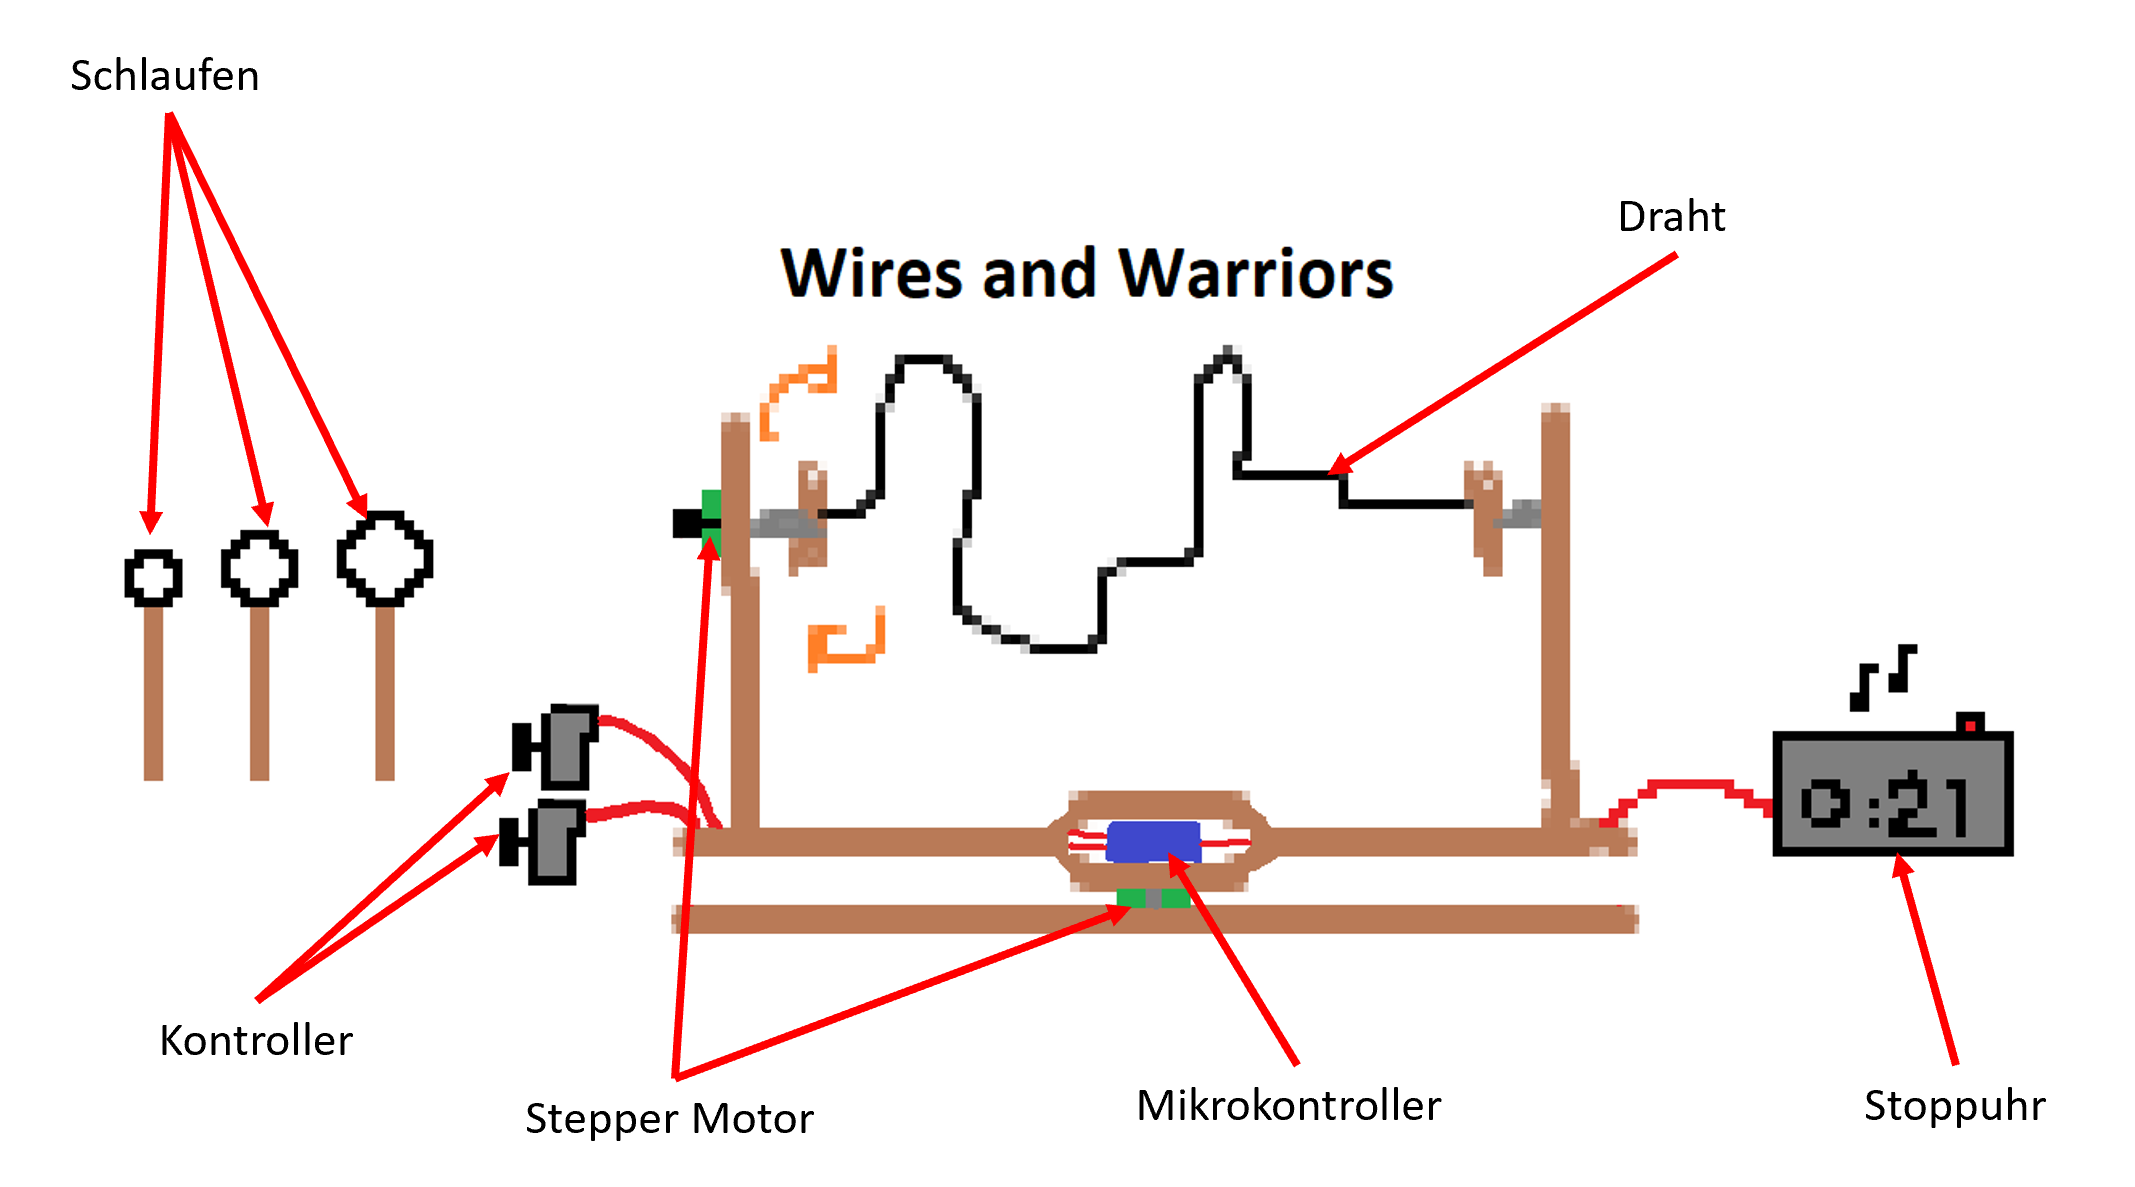
\includegraphics[width=0.75\textwidth,scale=1]{./images/Konzeptpapier_1.png}}
 \caption{Visualisierung des ersten Konzepts}\label{imageLabel}
\end{figure}  

\textbf{Zweite Konzept}: Dieses System sollte drei separate Drähte nutzen: einer rechts, einer links und einer in der Mitte als Brücke. Die äußeren Drähte sollten sich um die Y-Achse und das Mittelstück um die X-Achse drehen können. Das Ziel ist es gewesen, die gegenüberliegende Seite zu erreichen. Die Herausforderung bestand darin, dass die Spieler sich koordinieren mussten, um das Spiel zu beenden. Dieses Konzept war nicht ausgereift, jedoch bietet sie ein vielversprechendes Grundkonzept für die weitere Entwicklung. Der Entwurf des Systems sah wie folgt aus:

\begin{figure}[H]
 \centerline{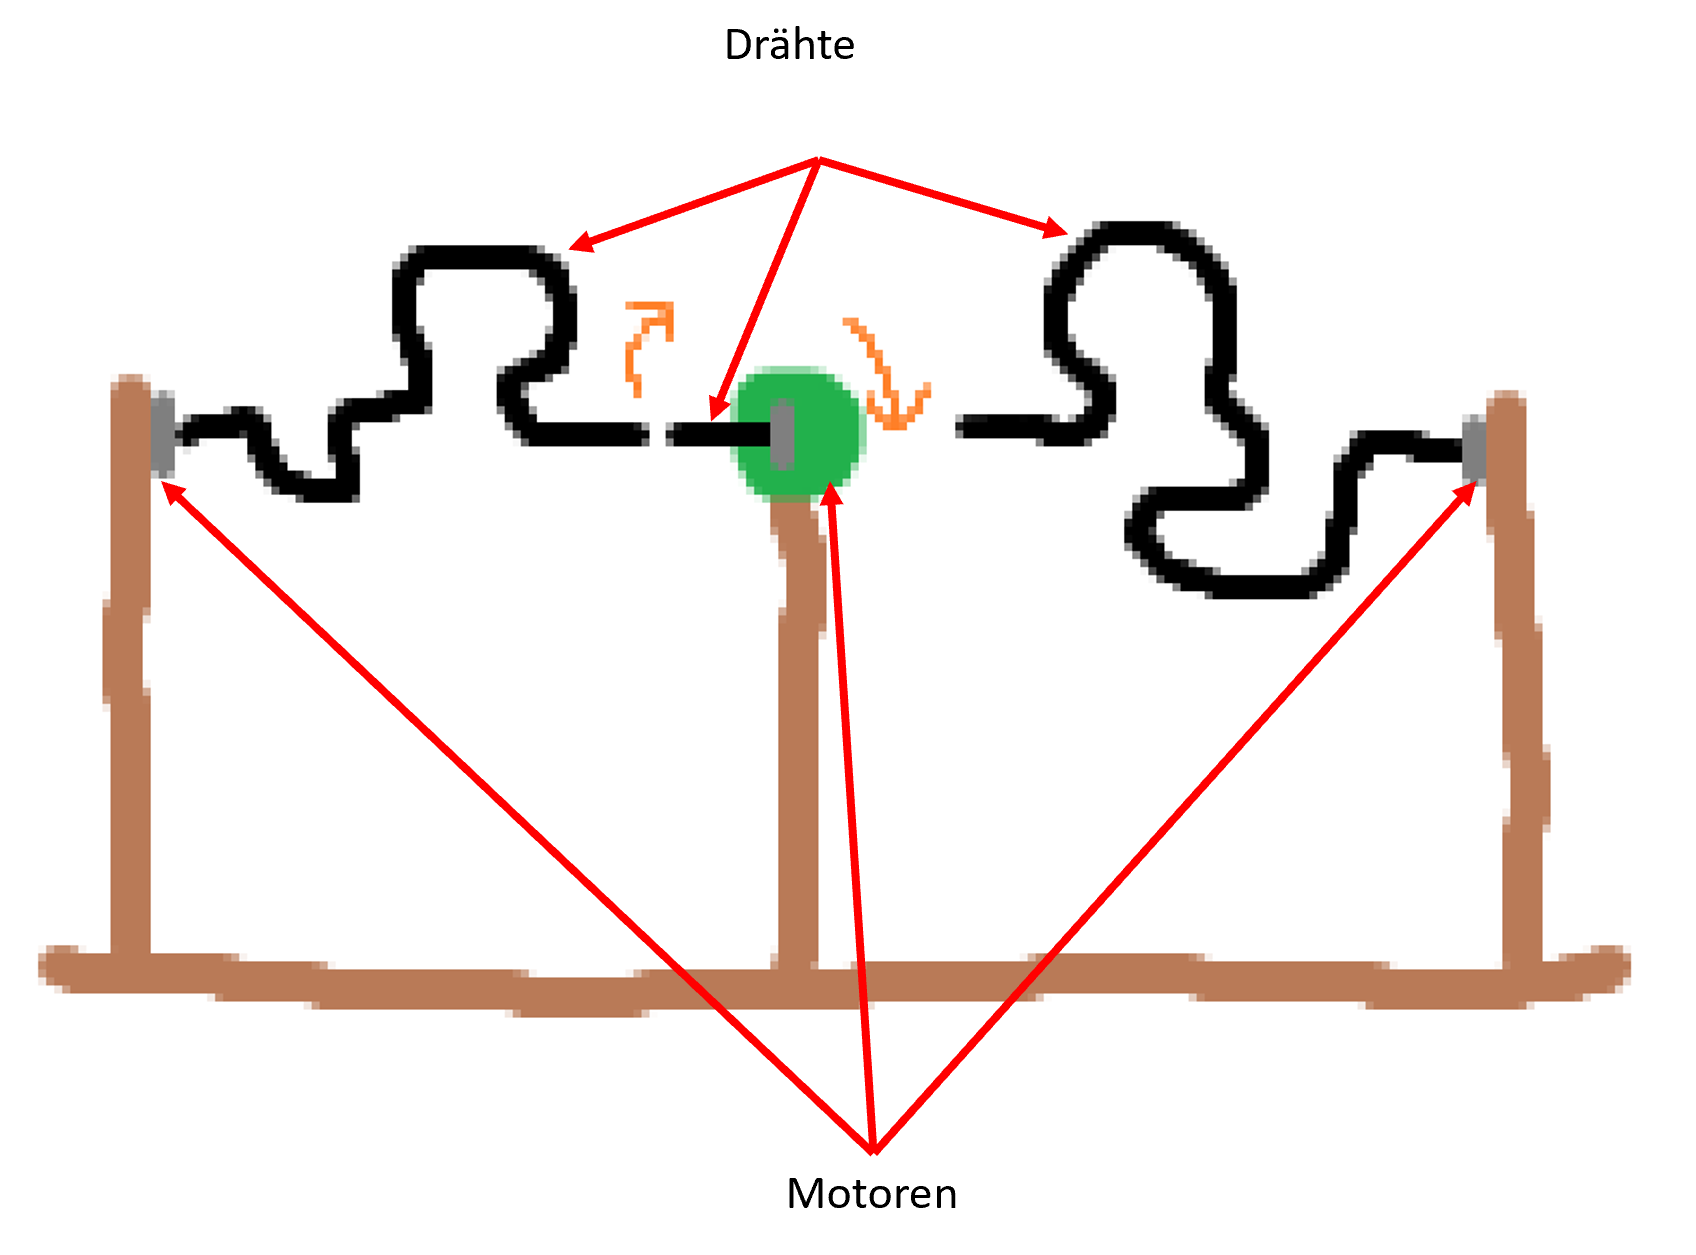
\includegraphics[width=\textwidth,scale=1]{./images/Konzeptpapier_2.png}}
 \caption{Visualisierung des zweiten Konzepts}\label{imageLabel}
\end{figure} 


\textbf{Dritte Konzept}: Das dritte Konzept sollte zwei Drähte besitzen. Diese wurden von den Seiten bis zur Mitte gespannt und am Mittelturm befestigt werden. Beide Spieler mussten, jeweils von den äußeren Seiten in die Mitte gelangen. Es zusätzlich möglich gewesen das ein dritter Spieler das System kontrollieren konnte über Kontroller. Diese Kontroller haben es ihm ermöglicht, die zwei Drähte rotieren zu lassen. Dieses Konzept entsprach nicht dem Charakter eines Escape-Rooms und wurde verworfen. Der Entwurf des Systems sah wie folgt aus: 

\begin{figure}[H]
 \centerline{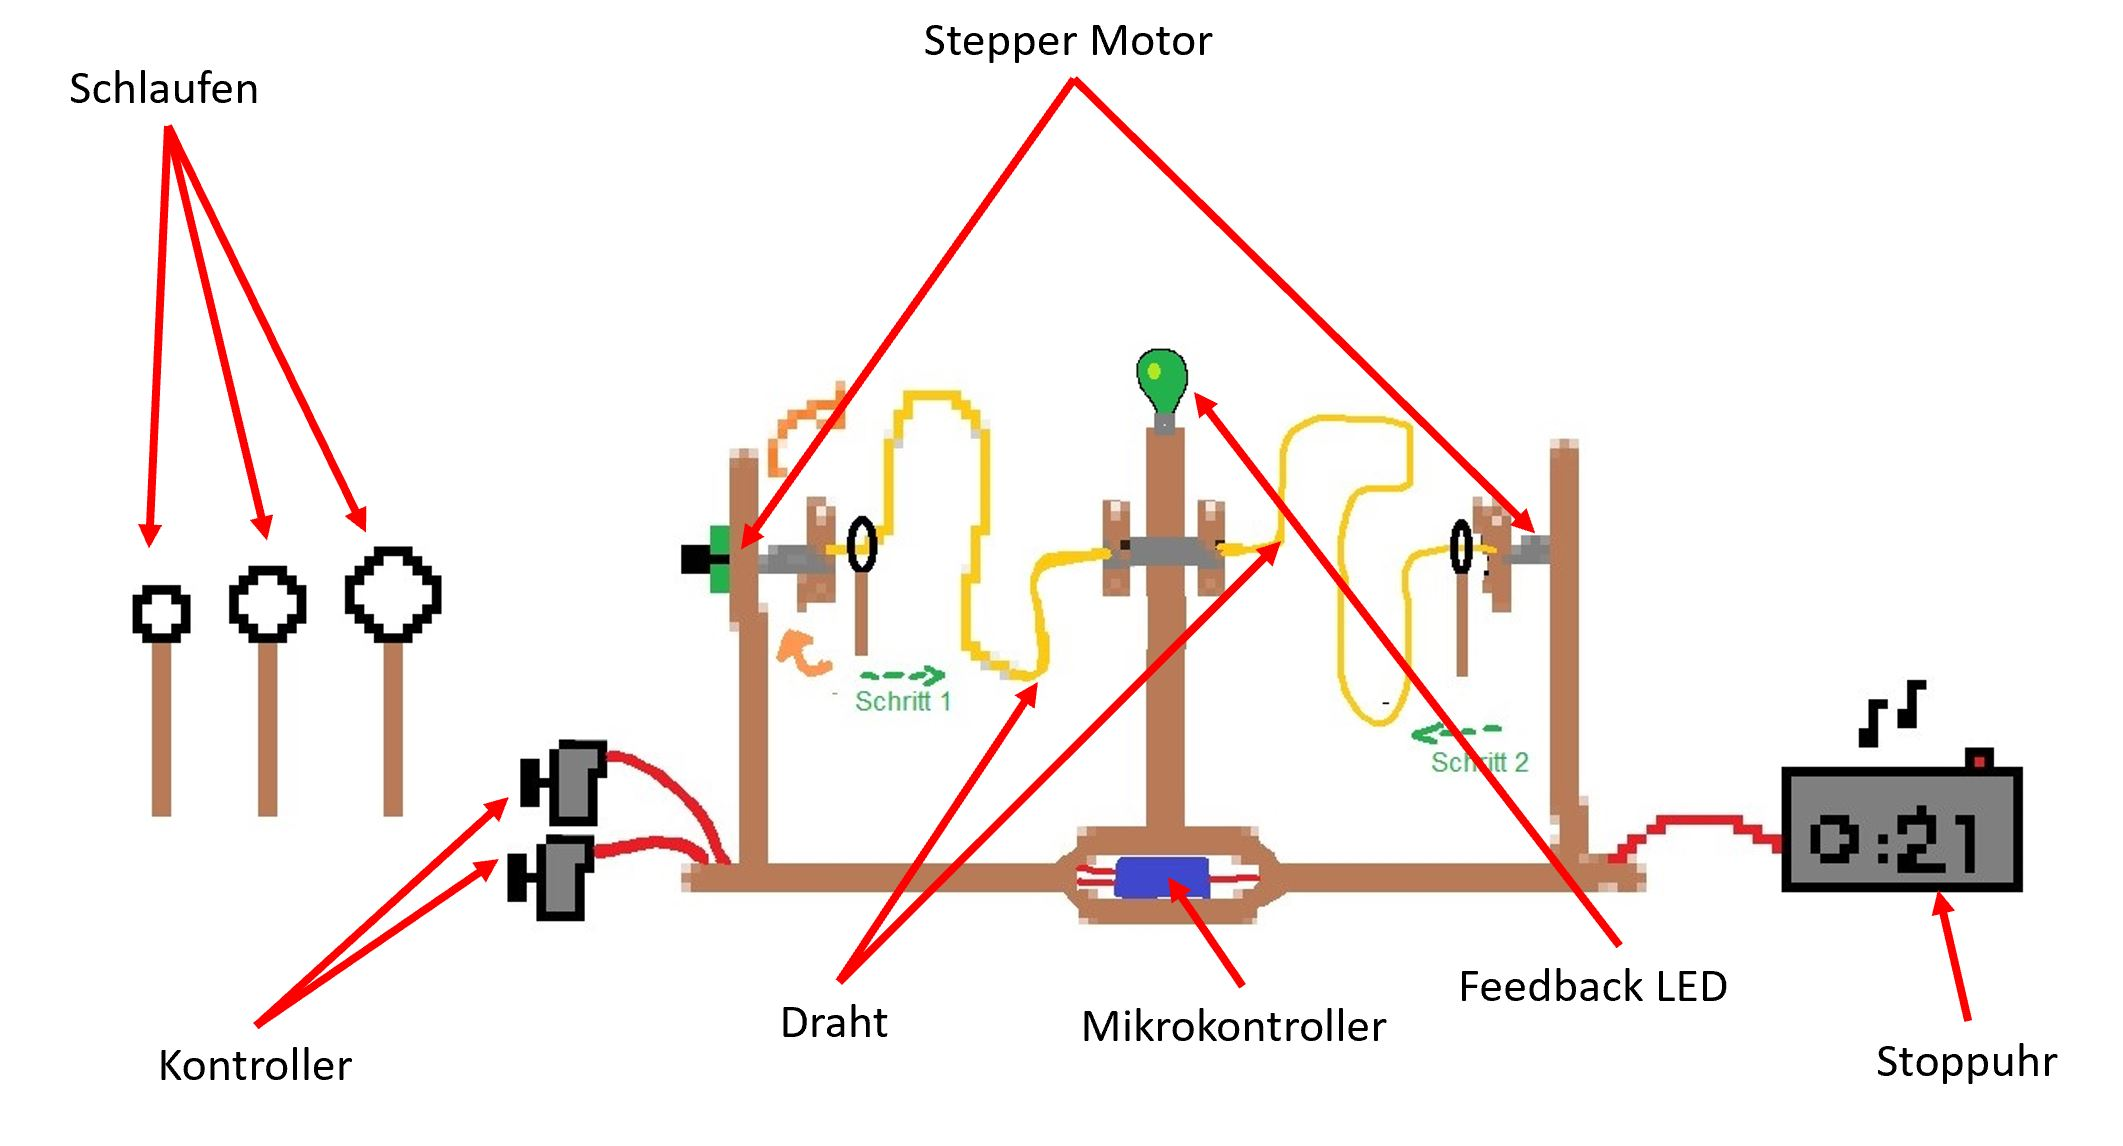
\includegraphics[width=\textwidth,scale=1]{./images/Konzeptpapier_3.jpg}}
 \caption{Visualisierung des dritten Konzepts}\label{imageLabel}
\end{figure} 


\textbf{Vierte Konzept}: Dieses Mal wurden die Türme auf einer Seite und die Brücke gegenüber platziert. Die Drahttürme rotieren um die Y-Achse und die Brücke um die X-Achse. Diese Idee wurde aufgrund mangelnder Nutzerfreundlichkeit schnell verworfen, jedoch wurde das Konzept des äußeren Gerüsts für das finale Design als Basis genutzt. Der Entwurf des Systems sah wie folgt aus:

\begin{figure}[H]
 \centerline{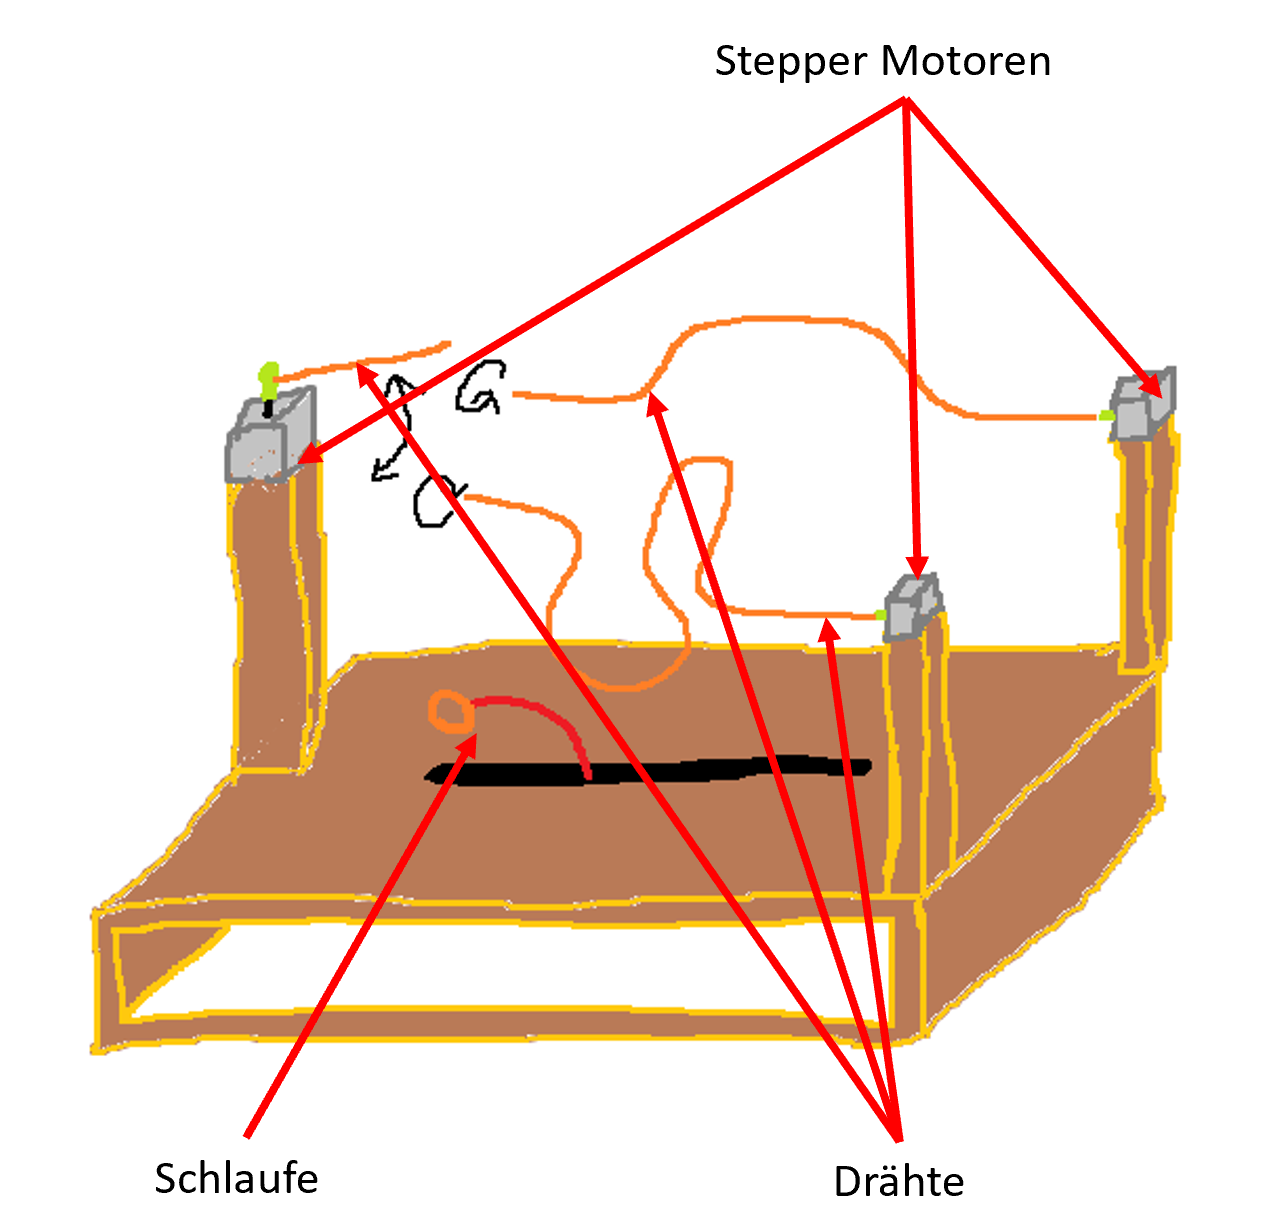
\includegraphics[width=.6\textwidth,scale=1]{./images/Konzeptpapier_6.png}}
 \caption{Visualisierung des vierten Konzepts}\label{imageLabel}
\end{figure} 

\textbf{Fünfte Konzept}: Das letzte Konzept ist eine Kombination aus dem dritten und zweiten Ansatz gewesen. Es gibt zwei Spieler, die gegen das System antreten, mit drei Drähten: links, rechts und ein Mittelstück. Die äußeren Drähte drehen sich um die Y-Achse, das Mittelstück um die X-Achse. Das System sollte ein Startknopf, Fehler-LEDs und Herzen zur Spieler-Rückmeldung besitzen. Die Spieler starten an den äußeren Türmen und müssen auf die andere Seite gelangen. Dieses Konzept war erfolgversprechend und wurde als Grundkonzept genommen und ausgearbeitet. Der Entwurf des Systems sah wie folgt aus:

\begin{figure}[H]
 \centerline{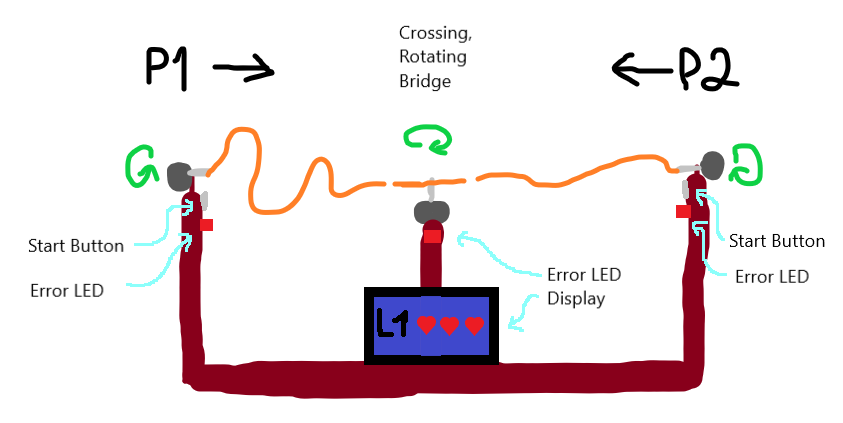
\includegraphics[width=\textwidth,scale=1]{./images/Konzeptpapier_5.png}}
 \caption{Visualisierung des fünfte Konzepts}\label{imageLabel}
\end{figure} 

\section{Modellierung des 3D-Design}

Bei der Modellierung des 3D-Designs für Wire \& Warriors wurde auf ein modulares System geachtet. Die Modularität war ein zentraler Aspekt des Designs, denn dadurch war es möglich die Komponenten für Wartung und Upgrade leicht zugänglich zu machen.

Das gesamte Gerüst des Spieles musste aufgrund der Größenbeschränkung der Holzplatten, jeweils 30x60 Zentimeter groß, durchdacht werden. Die Verwendung von Verzahnung im Modell war ein wichtiger Bestandteil. Diese Bauweise ermöglicht es, dass einzelne Platten fest eineinander greifen konnten, wodurch eine stabile Struktur ohne zusätzliche Verbindungselemente wie Schrauben oder Nägel zu schaffen. Diese Verzahnung sahen wie folgt aus:


\begin{figure}[H]
 \centerline{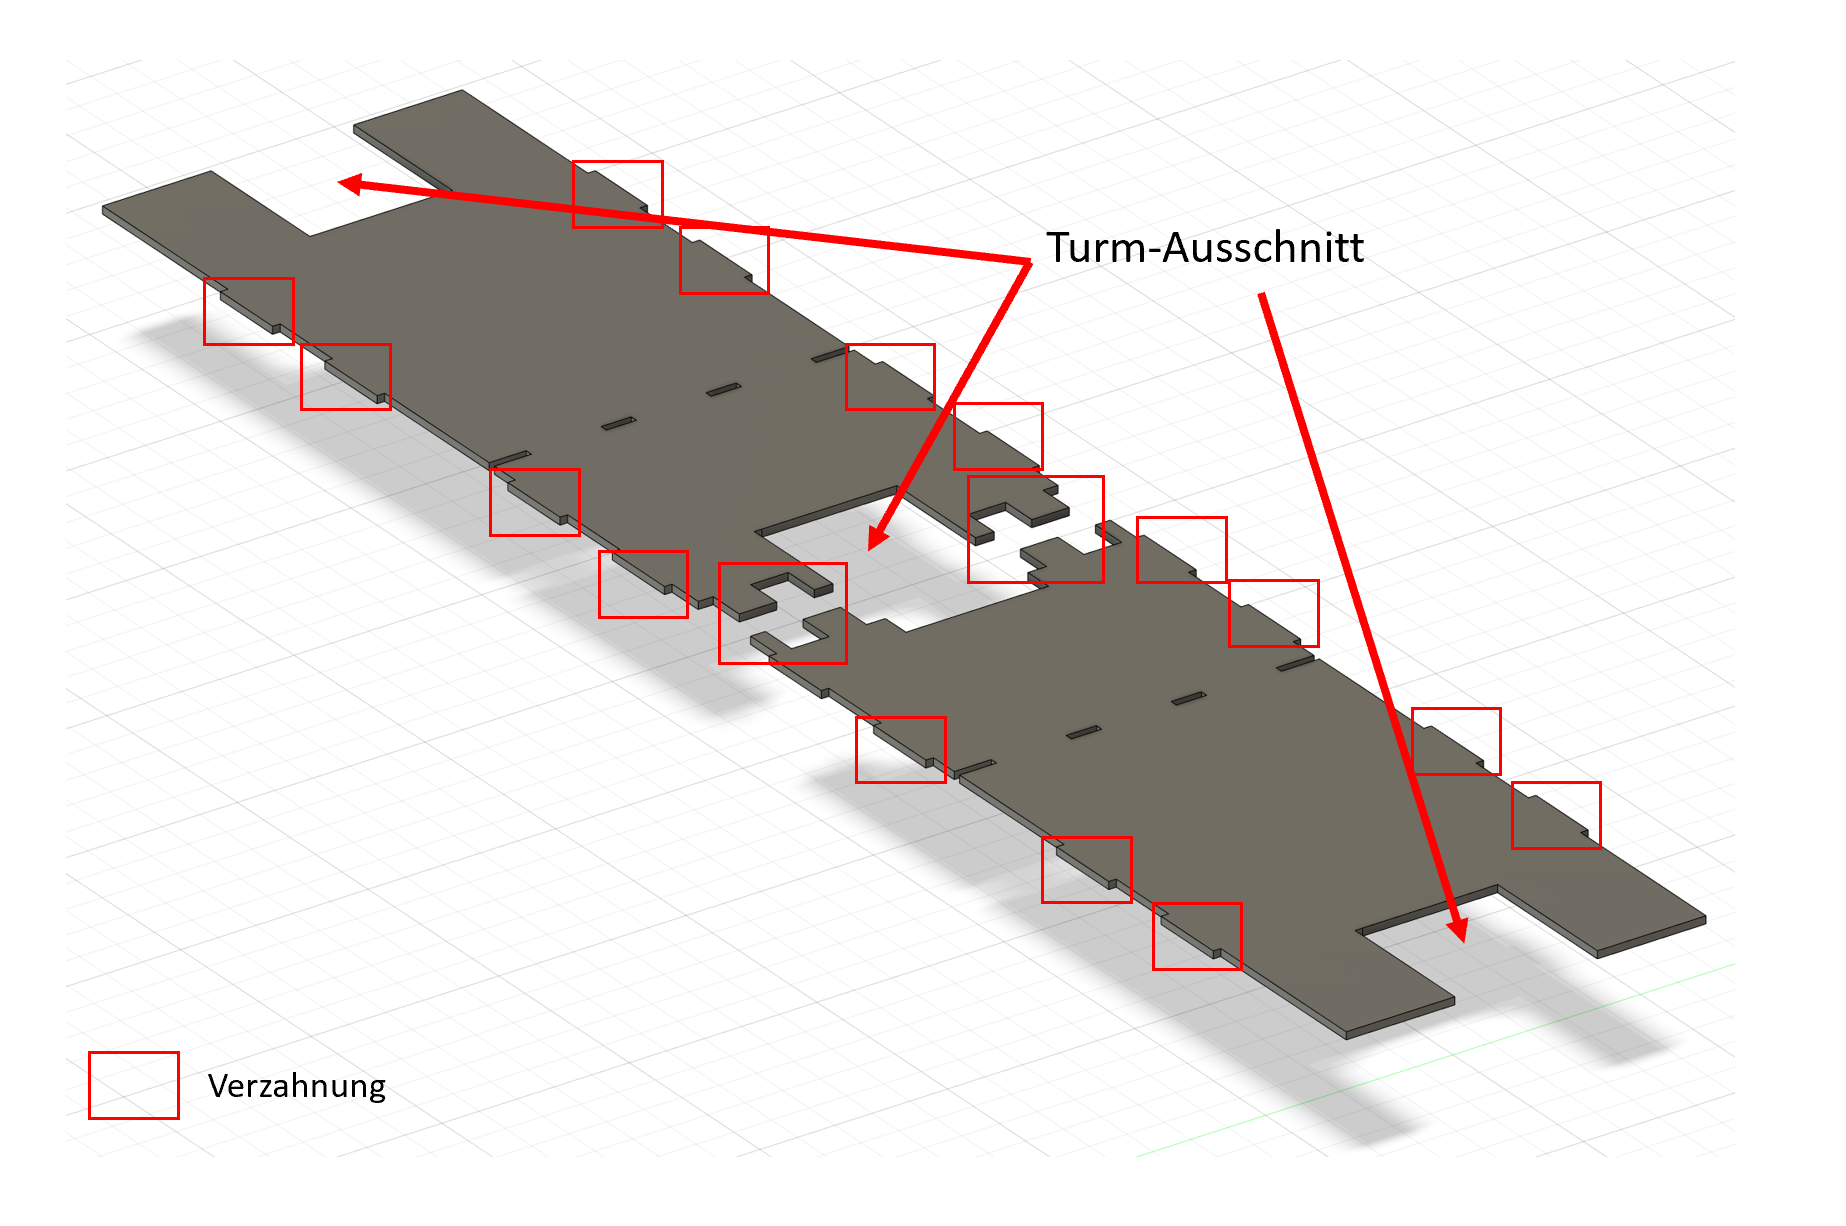
\includegraphics[width=\textwidth,scale=1]{./images/verzahnung.png}}
 \caption{Verzahnung am Deckel}\label{imageLabel}
\end{figure} 

Zusätzlich wurde des gesamt Gerüst durch die Mittelstücke, die auch als Kabelführung gedient haben, verstärkt. Die Mittelstücke wurden im Deckel, in den Wänden und am Boden angebracht. Diese Mittelstücke sehen wie folgt aus:

\begin{figure}[H]
 \centerline{\includegraphics[width=0.75\textwidth,scale=1]{./images/mittelstück.png}}
 \caption{Stabilisierung des Gerüstes durch Mittelstücke}\label{imageLabel}
\end{figure} 

Die Türme des Spieles wurden in das Gerüst eingesetzt und wurden durch die Deckel befestigt. Jeder Turm hatte einen Ausschnitt für den Stepper-Motor und eine Ablage. Die Türme sahen wie folgt aus:

\begin{figure}[H]
 \centerline{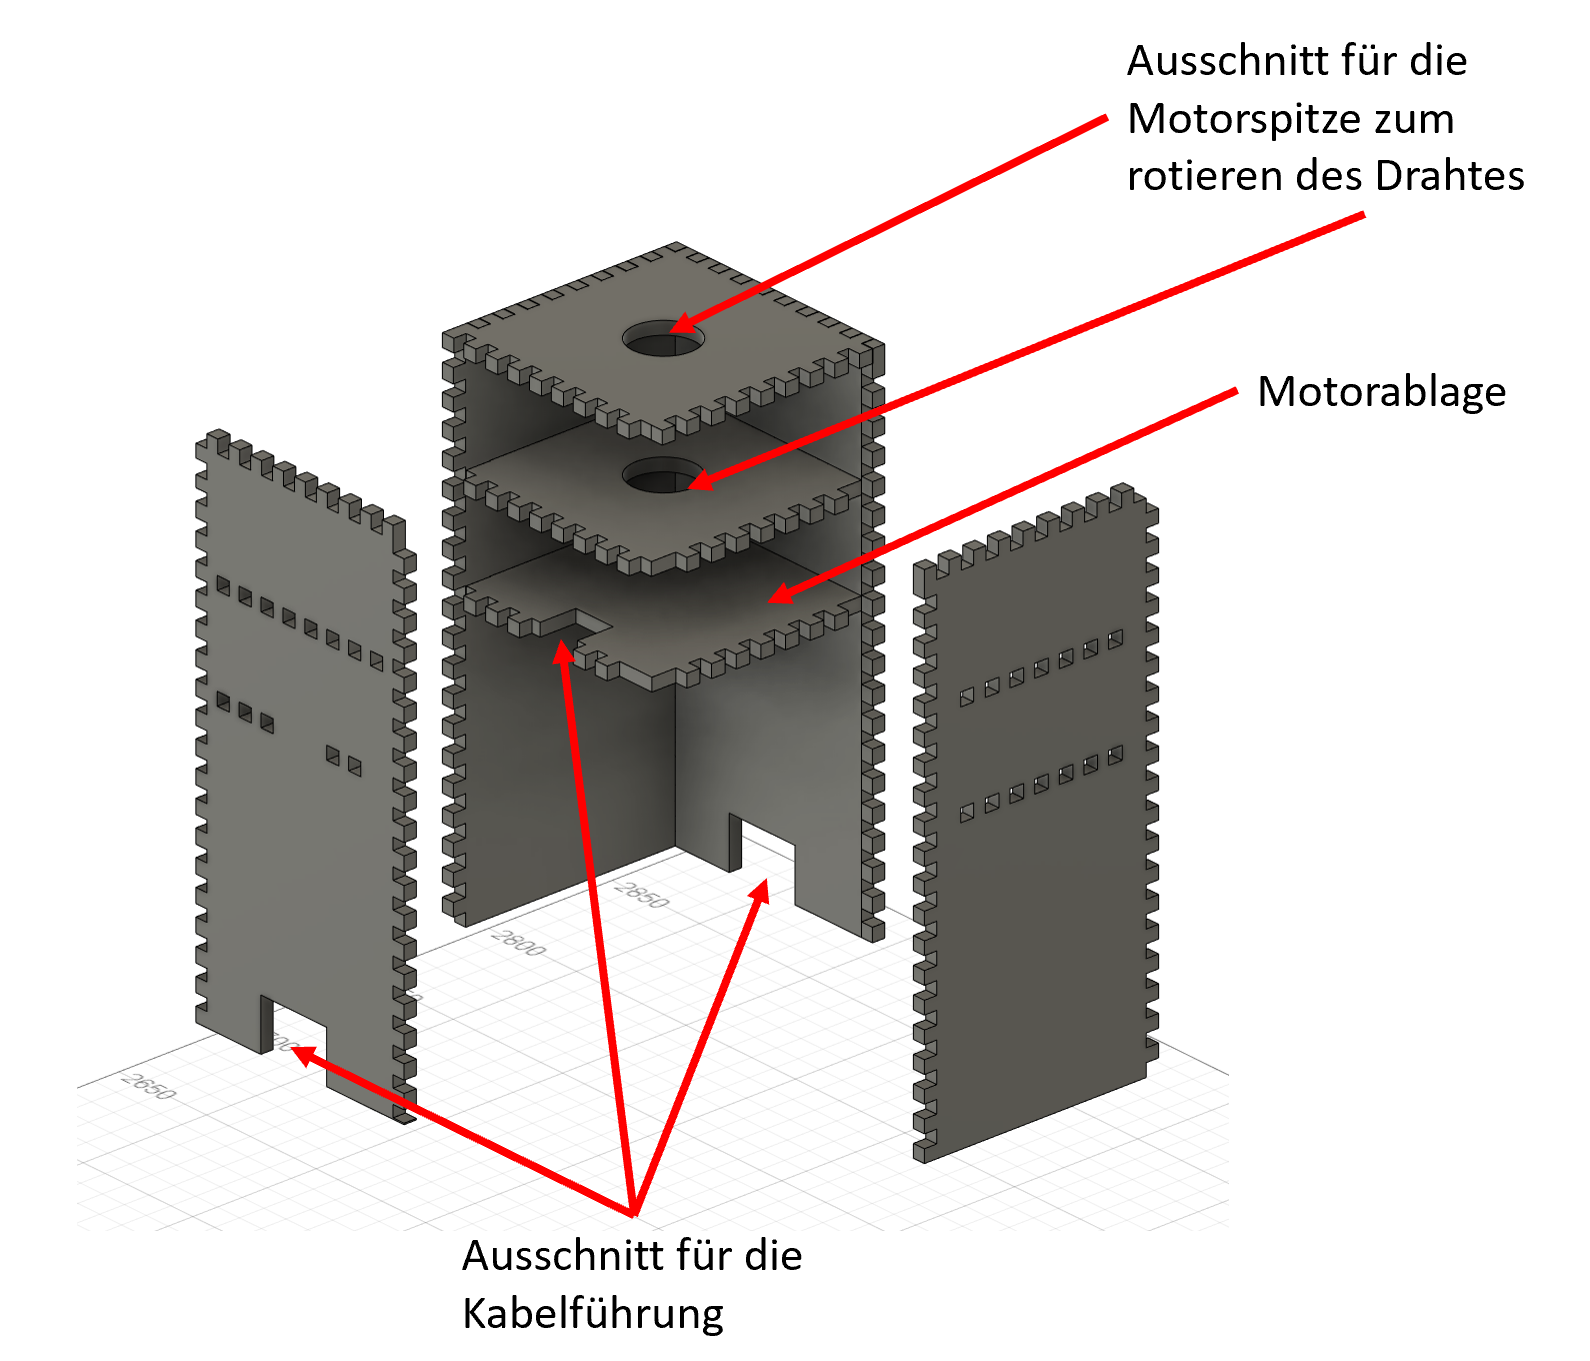
\includegraphics[width=0.75\textwidth,scale=1]{./images/turm_mitte.png}}
 \caption{Einblick in den mittleren Turm}\label{imageLabel}
\end{figure} 


Das gesamte Design diente als Vorlage für die Laserauschnitte, die später aus den Holzplatten gefertigt wurden. Diese Vorbereitung ist entscheidend gewesen, damit alle Teile Präzise zusammenpassen. 

Die Modularität und die leichte Zugänglichkeit der Komponenten sorgt für eine einfach Wartung bzw. Upgrades. Das hat den Vorteil, dass eine schnelle Anpassung z.B. an neue Spielvariaten möglich wäre. Das Endresultat ist ein durchdachtes und funktionales 3D-Design und sieht wie folgt aus: 

\begin{figure}[H]
 \centerline{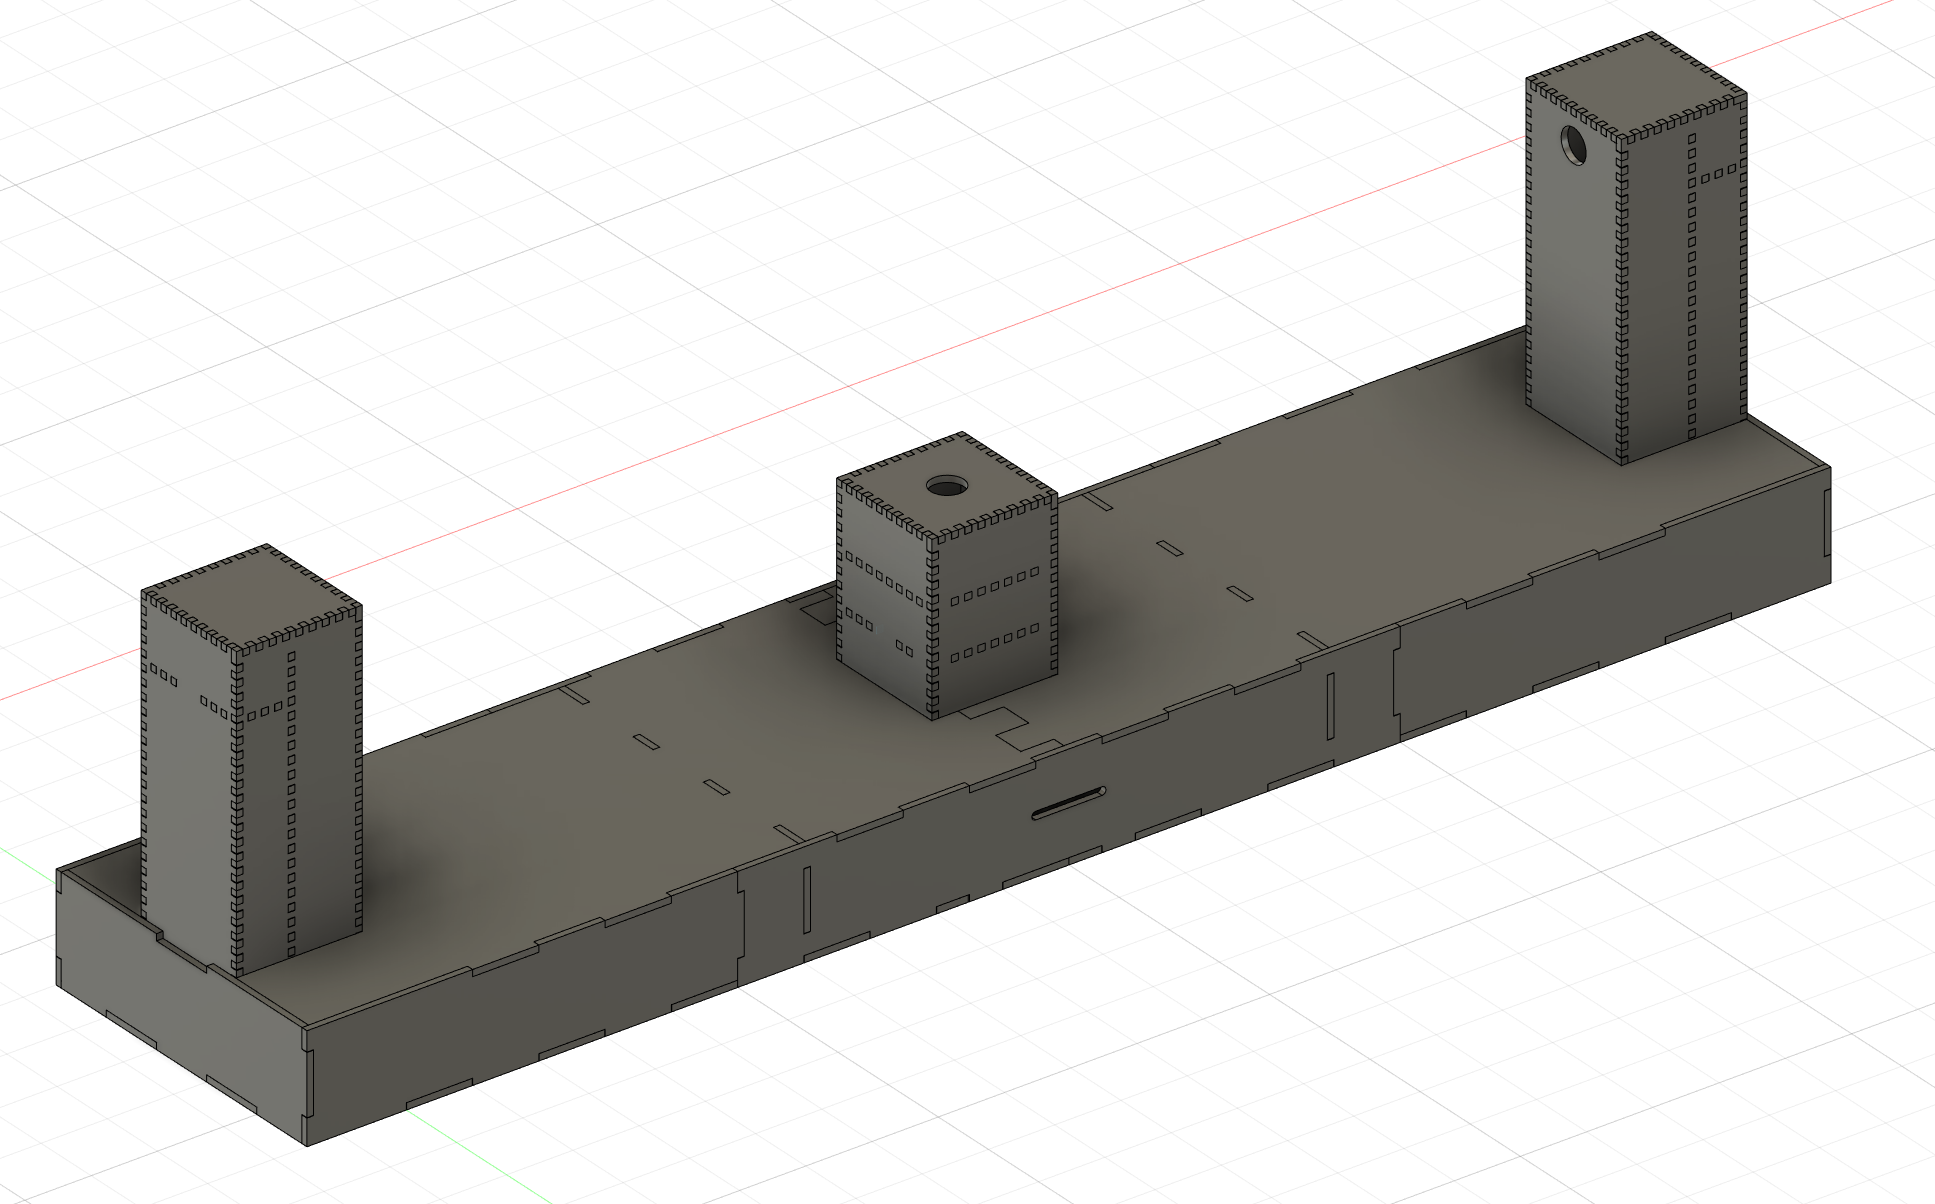
\includegraphics[width=\textwidth,scale=1]{./images/gesamt_design.png}}
 \caption{Das gesamte Design für Wire \& Warriors}\label{imageLabel}
\end{figure} 


  % ... weitere Kapitel
 
  % Literaturverzeichnis
  \phantomsection
  \addcontentsline{toc}{chapter}{Literaturverzeichnis}
  \begin{thebibliography}{10}
    \bibitem{quelle1} Schreiberling, Tim: ,,Bestseller-Buch'', 1.~Auflage, S.~13ff, Renner-Verlag, Musterstadt, 2011.
  \end{thebibliography}
  \newpage
  
  % Anhang
  \phantomsection
  \addcontentsline{toc}{chapter}{Abbildungsverzeichnis}
  \listoffigures
  \newpage

  \phantomsection
  \addcontentsline{toc}{chapter}{Tabellenverzeichnis}
  \listoftables
  \newpage
  
  %\include{anhang}
\end{document}  
